\chapter{Study 2 - Attentional Networks}
\label{ch:attentional}
To help simplify the learning problem the task was again reframed to improve the signal to noise ratio.
The preprocessing was adjusted such that frames were accumulated around every 150th event and instead of using the full image only an 11x11 frame was kept.
In keeping with previous experiments accumulation was applied into the past and future to be the input and output. 
Figure \ref{fig:11inoutpair} is an example of such a pair.
%Rather than applying decay to the whole image at uniform time intervals and using that as input the to the network each event was decayed around resulting in many more (albiet similar) training examples.
%However only an 11x11 area around each event was considered meaning the signal to noise ratio was much higher. 

\begin{figure}[h]
    \centering
    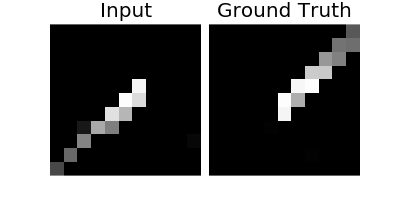
\includegraphics[width=0.8\textwidth]{11xinoutpair_83.png}
    \caption{Example of 11x11 input for an attentional network}
    \label{fig:11inoutpair}
\end{figure}

Figure \ref{fig:11inoutpair} is a cherry picked training example.
The Attentional networks still had a noisy task to solve because all events, including noise events, are considered. 
Many of the training examples derived from noise pixels could have been filtered out efficiently by demmanding the total activity in a training example excede some low threshold.
However, the system should be able to deal with noise and setting such a threshold would create another unnecessary hyper-parameter to the model.
Additonally such a parameter would be dependent on the time scale of the data and would need to be adjusted for each task. 
As will be shown the network was able to learn even in the midst of such noise so it was left in. 

%%%%%%%%%%%%%%%%%%%%%%%%%%%%%%      ATTENTIONAL NN    %%%%%%%%%%%%%%%%%%%%%%%%%%%%%%%%%%%%%%
\section{Attentional Directly Connected (ADC) Network}

\subsection{Aims}
% TODO Need to actually set some aims here
The network, as the name suggests, is a direct connection between the input and output units with no hidden layer.
The prediction problem had been broken down into a seemingly simple task so it was expected that results could be achieved with a simple network now the signal-to-noise ratio was larger within training examples.

\subsection{Method}
The network details are outlined in table \ref{tb:attnet1def}, with key points being the loss function has returned to the standard S.S.D. instead of the linearly weighted S.S.D. and the number of inputs has drastically decreased. 

\begin{table}[h]
\centering
\begin{tabular}{ | l | l | }
    \hline
    Num. Inputs & 121 \\
    Num. Outputs & 121 \\
    Connectivity & Fully connected \\
    Num. Hidden Layers & 0 \\
    Activation function & Linear, ReLU, Sigmoid \\
    Loss & Sum of Squares Difference \\
    Learning rule & S.G.D. (back propogation) \\
    Learning rate & 0.1 \\
    Mini-batch size & 100 \\
    \hline
\end{tabular}
\caption{Features of the Attentional Directly Connected Networks}
\label{tb:attnet1def}
\end{table}

\subsection{Linear activation}
The simplest ADC network considered had only a linear activation to compute outputs. 
This proved to be enough for the network to learn to make coherent predictions. 
The two datasets (8 Angle and Arbitrary Angle) were considered, a network was trained on each and then made predictions on a set of validation data from it's own dataset and other dataset to see how it could generalise.
For clarity the networks trained on the 8AD will be called 8AngNets and the networks trained on the AAD will be called ArbAngNets. 

\subsubsection{Linearly activated 8AngNet results}

\begin{figure}
    \centering
    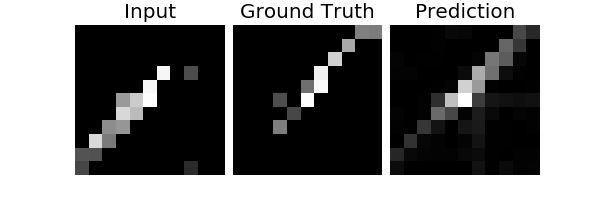
\includegraphics[width=0.8\textwidth]{ADC_8a_8a_13.png}
    \caption{A reasonable prediction from 8AngNet on the 8AD validation set.}
    \label{fig:ADC_8a_8a_crct} 
\end{figure}

\begin{figure}
    \centering
    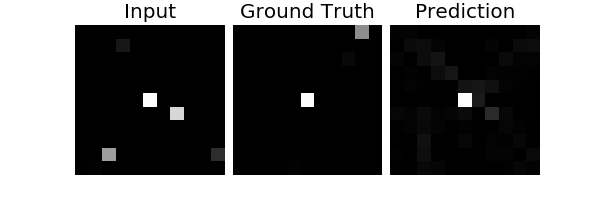
\includegraphics[width=0.8\textwidth]{ADC_8a_8a_7.png}
    \caption{A prediction from 8AngNet with a noisy input}
    \label{fig:ADC_8a_8a_noisy}
\end{figure}

Figures \ref{fig:ADC_8a_8a_crct} and \ref{fig:ADC_8a_8a_noisy} show how the linearly activated 8AngNet predicted in two cases from the 8 Angle validation set.
This prediction looks promising that the network is capable of representing some structure of the data as the prediction is similar to the label (ignoring some noise).
% TODO Make this an even more correct image and use this particular img (13) later to discuss problems
%In figure \ref{fig:ADC_8a_8a_crct} the network is performing well and gives a prediction which is quite similar the ground truth (ignoring noise). 
Figure \ref{fig:ADC_8a_8a_noisy} shows a noisy training example.
The label does not intuitively follow from the input and the network only outputs small values.
However the network does predict faintly along the North-West diagonal which is sensible when considering the input has two pixels along the South-East diagonal (the closer of which is highly active making it resemble a decayed path). 
%However the network has noticed two pixels active along the bottom right diagonal (one of which is highly active) and the network predicts a faint output along the top left diagonal.

\begin{figure}
    \centering
    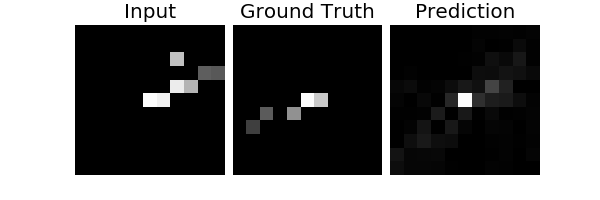
\includegraphics[width=0.8\textwidth]{ADC_8a_aa_4.png}
    \caption{8AngNet struggles to predict AAD examples}
    \label{fig:ADC_8aNoaa}
\end{figure}

\begin{figure}
    \centering
    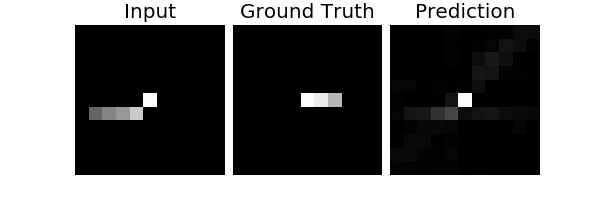
\includegraphics[width=0.8\textwidth]{ADC_8a_aa_46.png}
    \caption{8AngNet predicting a slightly off angle input}
    \label{fig:ADC_8aNoaa_fork}
\end{figure}

The network performing well on its own validation set is a success in itself but raises the question of how it will generalise from 8AD to AAD.
It was hypothesised the network might be able to use a combination of known angles to represent the new angles in the Arbitrary Angle dataset.
This was not the case though, figure \ref{fig:ADC_8aNoaa} shows the network stuggling to predict the motion.
Most of the activity in the prediction falls in the East North-East section which is where the input was.
There is some very limited activity that matches the label but this is insignificant compared to previous predictions and what can be realistically expected from the network. 
Further figure \ref{fig:ADC_8aNoaa_fork} shows a slightly off center input which resembles an angle from 8AD. 
The network has trouble interpreting this and makes 3 very faint predictions being the North-East diagonal, the East edge and along the input.
This suggests the network is not able to efficiently represent the arbitrary angles as some combination of the angles it learnt and must be using some other internal representation such as mapping between regions.

An additional interesting case which supports a region mapping hypothesis is seen in figure \ref{fig:ADC_8aNoaa_special} in which the network suffering from some neatly aligned noise. 
The network is well equipped to deal with inputs coming from one angle at a time but this noise makes it appear as if two dots may be crossing paths. 
The networks behaviour to predict two strong output paths shows that each input path (and its predictions) are happening (at least somewhat) independently of the rest of the input.
If the network was representing the input as an angle it would be reasonable to expect that the output might be a blur in the North-East corner of the prediction.  
Instead this clear prediction of two paths suggests the network is simply learning to map between areas of the input to areas of the output. 

\begin{figure}
    \centering
    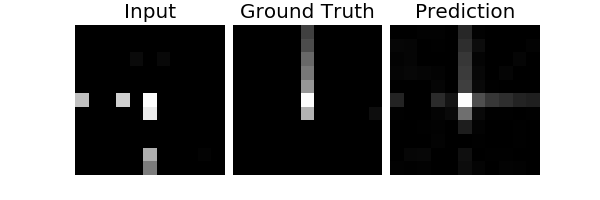
\includegraphics[width=0.8\textwidth]{ADC_8a_aa_15.png}
    \caption{8AngNet network predicting two paths due to noise}
    \label{fig:ADC_8aNoaa_special}
\end{figure}


\subsubsection{Linearly activated ArbAngNet results}
It follows that a network trained on only 8 angles would have trouble generalising to arbitrary angles so a second network was trained on the Arbitrary Angles Dataset. 
In general the network trained on Arbitrary Angle data was less confident in its predictions (magnitude of predictions were lower) but in each guess it would cover a boarder area. 
% TODO rewrite this sentence
An example of this is figure \ref{fig:ADC_aaaa_crct} in which the prediction has many faintly coloured squares, in contrast to the more confident predictions made in figure \ref{fig:ADC_8a_8a_crct} by 8AngNet.

\begin{figure}[h]
    \centering
    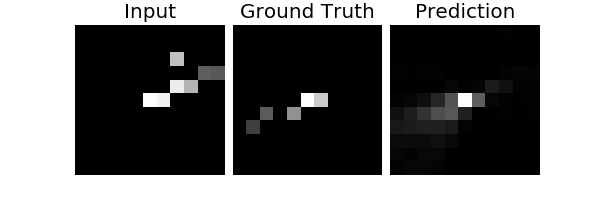
\includegraphics[width=0.8\textwidth]{ADC_aa_aa_4.png}
    \caption{ArbAngNet correctly predicting}
    \label{fig:ADC_aaaa_crct}
\end{figure}
% TODO these visualisations can be improved by grouping the predictions from both nets into 1 img


\begin{figure}[h]
    \centering
    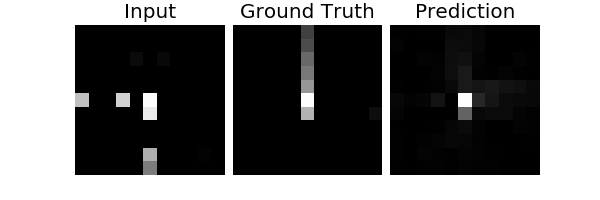
\includegraphics[width=0.8\textwidth]{ADC_aa_aa_15.png}
    \caption{ArbAngNet predicting two paths due to noise}
    \label{fig:ADC_aaaa_twopath}
\end{figure}

\begin{figure}[h]
    \centering
    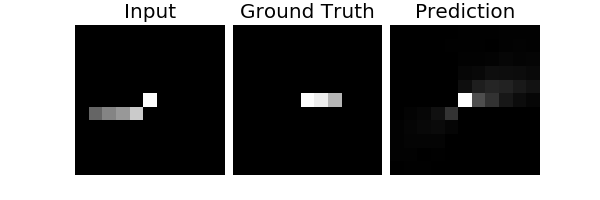
\includegraphics[width=0.8\textwidth]{ADC_aa_aa_46.png}
    \caption{ArbAngNet predicting a slightly off angle input}
    \label{fig:ADC_aaaa_fork}
\end{figure}


The neat noise example which suggested that 8AngNet was simply mapping regions in the input to regions in the output shows a very different prediction from ArbAngNet.
ArbAngNet does not predict any given angle strongly but instead has a very faint prediction along both but also between the two lines. 
The significance of these prediction is questionable given how small the predictions are but it does give some insight into the networks dynamics.
It should be noticed that this does not exclude the possibility that ArbAngNet is also just mapping between regions of the input and output, rather this is still a promising theory.
Finally, figure \cite{fig:ADC_aaaa_fork} shows ArbAngNets performance on the slightly off angle example that 8AngNet failed to predict in figure \ref{fig:ADC_8aNoaa_fork}.

\subsection{Non-linear acitivation}
Compare Sigmoidal with relu?

\subsubsection{Sigmoid activation}
Talk about both 8AD and AAD here

\subsubsection{ReLU activiation}
Talk about both 8AD and AAD here 

\subsection{Attentional Directly Connected network discussion}
The ADC networks were successfully able to make meaningful predictions on both the 8AD and AAD datasets even with only a linear activation.
Neatly aligned noise suggests the networks internal representation is to map between pixels in the input to pixels in the output.
This is supported by 8AngNets inability to generalise to the AAD, naturally if the network hasnt learnt that a region (i.e. between two angles of 8AD) should map to another region than it will not be able to generalise to this. 
If the network had learnt to represent the training examples as angles then this generalisation should have been possible. 


%%%%%%%%%%%%%%%%%%%%%%%%%%%%%%      ATTENTIONAL NN    %%%%%%%%%%%%%%%%%%%%%%%%%%%%%%%%%%%%%%
\section{Attentional Hidden Layer (AHL) Network}

\subsection{Aims}
Following in the 

 using a hidden layer, what can learn? maybe line params, 1, 2, more hiddens

\subsection{Method}

\begin{figure}[h]
    \centering
    \includegraphics[width=1\textwidth]{AHLrelu.png}
    \caption{ReLU activated AHL network performance with varying hidden units}
    \label{fig:attnConvInvariant}
\end{figure}

\subsection{Results}


\subsection{Discussion}

%%%%%%%%%%%%%%%%%%%%%%%%%%%%%%      CONV NET    %%%%%%%%%%%%%%%%%%%%%%%%%%%%%%%%%%%%%%
\section{Attentional convolutional networks}
\subsection{Aims}
With positive results from the ADC and AHL networks the possibility of the convolutional networks with the attentional training datasets was considered. 
The simple, regular structure in the attentional training data might be enough for a shallow convolutional network to learn. 

\subsection{Method}
The network structure, methodology and manipulated variables were identical to that in section \ref{sec:convMethod} with some minor differences.
These differences included the change in input/output size from 16384 to 121 and convolution size from 11x11 to 6x6. 
The input/output layer size change was necessary given the smaller size of the training examples and the convolution size change was considered given the input was now only 11x11.
As the attentional accumulation trims the training examples to 11x11 then in theory each temporal past/future should only take up a 6x6 grid. 

\subsection{Results}
Despite the attentional data and the reduced size the convolutional networks still become input invarient as shown in figure \ref{fig:attnConvInvariant}.
The activity pattern shown is from the network using a size 8 dot moving with speed 4 accumulated with an exponential function and k value corresponding to a 33 ms period.
This invariance was consistant (although the given activity pattern would change) regardless the number/size of feature maps, the fully connect layer depth and fully connected layer activation.

\begin{figure}[h]
    \centering
    \includegraphics[width=0.7\textwidth]{attConvInvariance64.png}
    \caption{Attentional Convolutional Net showing input invariance.}
    \label{fig:AHLrelu}
\end{figure}

\subsection{Discussion}
The cause for this invariance in not known, the most promising explaination being a problem similar to the invariance seen in the PilotNets.
That is that the network quickly learns it can minimise the loss function by setting most values to zero and highlighting pixels based on frequency of appearing in the output.
For the PilotNets the frequent pixels were the hot pixels, for the attentional convolutional networks the frequent pixels are those near the center.
This explaination has trouble explaining why the convolutional networks would be unable to learn using the S.S.D. loss function when the ADC and AHL networks are able to make meaningful predictions using it.  

%%%%%%%%%%%%%%%%%%%%%%%%%%%%%%      AUTO ENCODE     %%%%%%%%%%%%%%%%%%%%%%%%%%%%%%%%%%%%%%
\section{Auto Encoder}
\subsection{Aims}
Noise has been accepted as a fact of neuromorphic sensors so far in this work and models have been expected to be able to deal with this.
A simple thresholding could have efficiently filter out many of the noise based training examples before use in training. 
Such a threshold would be dataset specific (with larger/faster dots creating more events) though and creates an unnecessary hyperparameter to the model. 
Instead noise could be filtered out using an Autoencoder.
This possibility is explored with autoencoders of various size.

\subsection{Methodology}
Simple Autoencoders consisting of a single fully connected hidden layer were used. 

\subsection{Results}

\begin{figure}[h]
    \centering
    \includegraphics[width=0.85\textwidth]{AEUnits.png}
    \caption{Effects of additional hidden units on AAD dataset Autoencoder}
    \label{fig:AEUnits}
\end{figure}


\subsection{Discussion}
 
